\chapter{Results} 

\section{Genetic Algorithm}

In the following results each test was repeated three times and averaged to give a better idea of the typical performance of the genetic algorithm approach.  Each test is categorized by the parameter that was changed as well as the reason and expected results of the changes to the parameters.  Also, with the exception of the bitstring segment length test, all other tests are conducted using the normal segment lengths (Table \ref{tab:geneticSegments}).  Lastly, for brevity only the SQL injection results will be compared across all test cases as it is the most complex request out of the three, a full listing of the graphical results for the other two attack types as well as complete text based results for all attack types is included (Appendix \ref{app:geneticFullResults}).

\subsection{Finding Best Parameters}

The performance and effectiveness of the genetic algorithm can be attributed to the parameters that are used and there is no universal choice for the parameters as it will always depend on the data set in question.\cite{optimalPopulationGenetic}  Each parameter of the genetic algorithm will affect the results in different ways, therefore it was important to first determine what settings would be most suitable to use for later tests so that those subsequent results would not be heavily influenced by the parameters instead of the independent variable being manipulated (Table \ref{tab:gaTestParameters}).  

\begin{table}[h]
	\centering
	\begin{tabular}{|p{1.5in}|p{0.675in}|p{0.675in}|p{0.675in}|p{0.675in}|p{0.675in}|}
	\hline
	\textbf{Test} & \textbf{Popul-ation} & \textbf{Gener-ations} & \textbf{Iter-ations} & \textbf{Muta-tion Rate} & \textbf{Elitist Pool} \\ 
	\hhline{|=|=|=|=|=|=|}
	\textbf{Population Size} & \textbf{$x$} & 100 & 1 & 0.5\% & 5\% \\
	\hline
	\textbf{\# of Generations} & 1250 & \textbf{$x$} & 1 & 0.5\% & 5\% \\
	\hline
	\textbf{Mutation Rate} & 1250 & 100 & 1 & \textbf{$x$} & 5\% \\
	\hline
	\textbf{Eltitist Pool} & 1250 & 100 & 1 & 0.5\% & \textbf{$x$} \\
	\hline
	\textbf{Multiple Iterations} & 1250 & 100 & \textbf{$x$} & 0.5\% & 5\% \\
	\hline
	\textbf{Bitstring Length} & 1250 & 100 & 1 & 0.5\% & 5\% \\
	\hline
	\end{tabular}
	\caption{Parameters used in each Genetic Algorithm Test}
	\label{tab:gaTestParameters}
\end{table}

\subsubsection{Population Size} \label{sec:resPopulation}

\begin{wrapfigure}{r}{0pt}
	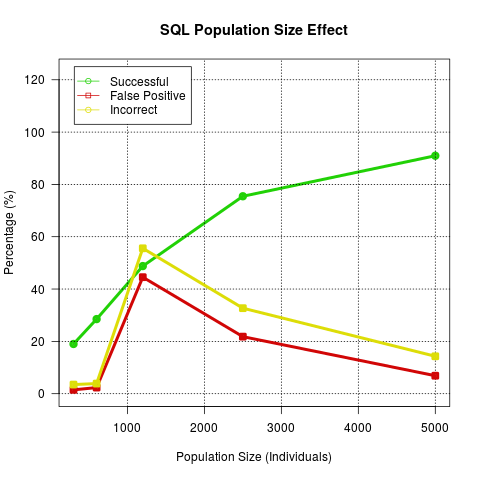
\includegraphics[width=250px]{./assets/results/ga/pop/Results_SQL.png}
	\caption{Effects of Population Size on Detecting SQLi}
	\label{fig:resPopSize}
\end{wrapfigure}

Population size is one of the most important parameters because a genetic algorithm with a low population size performs very poorly due to there not being a large enough sample size to grow and advance from.  Larger populations are more likely to generate new individuals that perform well however this also comes at a performance cost as every individual that is added is another individual that must have it's fitness evaluated.\cite{optimizationOfControlParameters}  In addition, for our purposes having a larger population increases the chances of having signatures that perform badly as well, causing increased false positives and incorrect detections.  In the worst case every attack in the testing set will be unique and require a new signature so a population size any less than that amount may miss attacks (Figure \ref{fig:resPopSize}).

\subsubsection{Generations} \label{sec:resGeneration}

The amount of generations also significantly matters because it is the amount of times the genetic algorithm will run.  The more generations the more likely that the algorithm can produce better results and improve upon the existing results (Figure \ref{fig:resGenerations}).

\begin{figure}[hb]
	\centering
	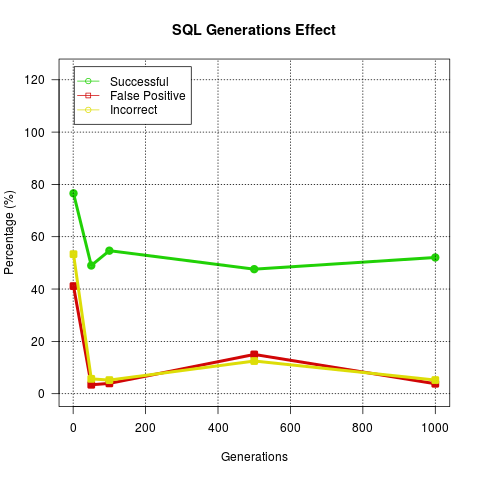
\includegraphics[width=350px]{./assets/results/ga/generations/Results_SQL.png}
	\caption{Effects of Generations on Detecting SQLi}
	\label{fig:resGenerations}
\end{figure}

\newpage
\subsubsection{Mutation Rate} \label{sec:resMutation}

If the mutation rate is too high then the genetic algorithm basically becomes a random search, while having no mutation rate at all will result in a lack of genetic diversity, with new bitstrings only being produced due to crossovers crossovers.  It is very difficult to determine a single mutation rate to get the best results and more often than not this is done by trial and error like the following tests will perform.\cite{aNewStrategy}  Mutation rates are typically set to a very low amount since it is on a per allele basis and you would not want to randomize every single bit in a signature and so a value between 0.0 and 1.0\% is often used with 1.0\% being quite high (Figure \ref{fig:resMutation}).\cite{optimizationOfControlParameters}

\begin{figure}[hb]
	\centering
	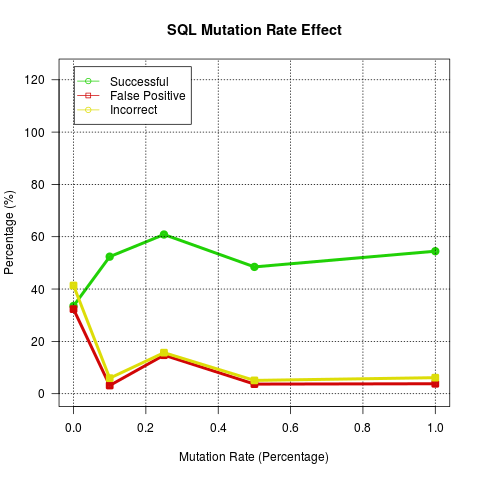
\includegraphics[width=350px]{./assets/results/ga/mutation/Results_SQL.png}
	\caption{Effects of Mutation Rate on Detecting SQLi}
	\label{fig:resMutation}
\end{figure}

\newpage
\subsubsection{Elitist Pool} \label{sec:resElitist}

The more of the better performing population that survives to the next generation the more likely that strong individuals will be selected to produce new individuals of similar strength.  However, if too much of the population is preserved than it may not be able to improve very quickly and the search may stagnate.  Sometimes this is also referred to as a generation gap (Figure \ref{fig:resElitist}).\cite{optimizationOfControlParameters}

\begin{figure}[hb]
	\centering
	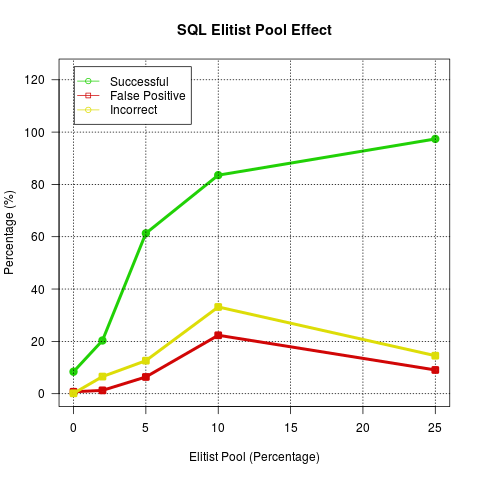
\includegraphics[width=350px]{./assets/results/ga/elitist/Results_SQL.png}
	\caption{Effects of Elitist Pool on Detecting SQLi}
	\label{fig:resElitist}
\end{figure}

\newpage
\newpage
\subsection{Combining Multiple Signature Sets} \label{sec:resIteration}

One of the claimed advantages of the genetic algorithm approach, and a big reason why it can work well is because the genetic algorithm can be used to produce new signatures in order to keep adding to an existing set to increase the breadth of detection.  For this reason, running the algorithm multiple times and combining the signatures should result in more detections, but may also result in increased false positives and incorrect detections due to many poor signatures being stored along with one another (Figure \ref{fig:resIterations}).

\begin{figure}[hb]
	\centering
	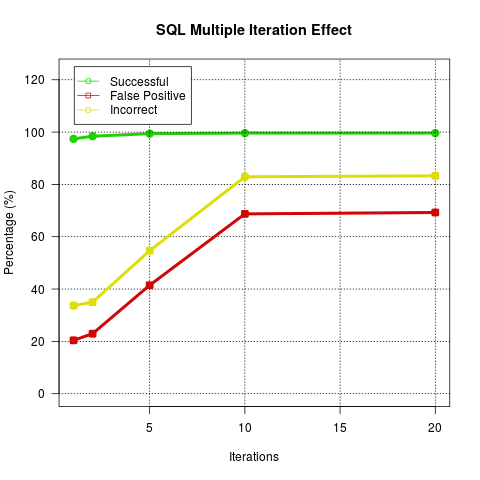
\includegraphics[width=350px]{./assets/results/ga/iterations/Results_SQL.png}
	\caption{Effects of Multiple Iterations on Detecting SQLi}
	\label{fig:resIterations}
\end{figure}

\newpage
\subsection{Bitstring Segment Length Effects} \label{sec:resSegment}

Because the genetic algorithm is able to detect additional attacks by generating new signatures, if the number of possible signature combinations is less thanks to the segment lengths, then it would be more likely to generate these signatures that match with the training or testing attacks.  However it also opens up the possibility of making it easier to generate poor signatures due to a smaller search space, as well as potentially artifically increase results due to segment overflows (Figure \ref{fig:resLength}).

\begin{figure}[hb]
	\centering
	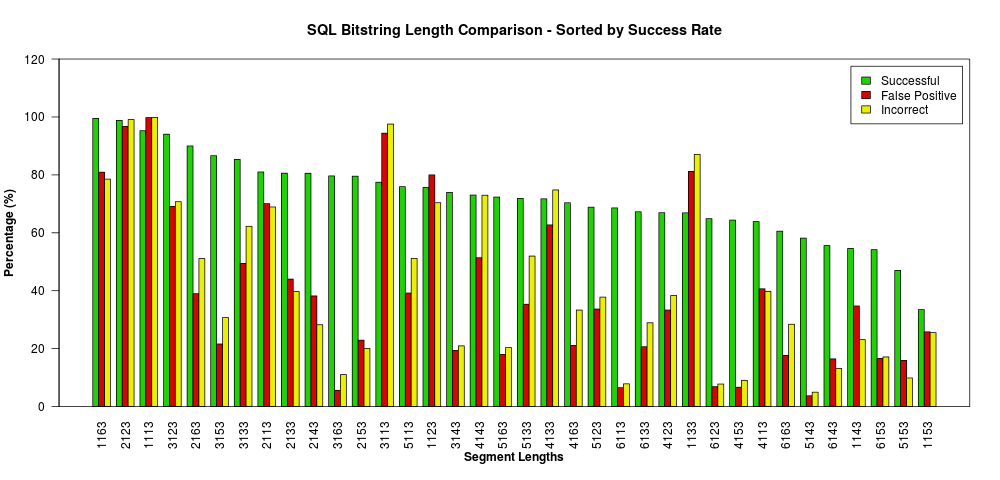
\includegraphics[width=450px]{./assets/results/ga/bitlength/Results_SuccessRate_SQL.png}
	\caption{Effects of Different Segment Lengths on Detecting SQLi}
	\label{fig:resLength}
\end{figure}

\newpage
\section{Compared With Random Permutations with Fitness} \label{sec:resRand}

The genetic algorithm approach works because of the ability to randomly generate new signatures using fitness to weed out the bad signatures so it would be very interesting to compare the approach with just simply generating all possible combinations and only using the bitstrings that performed well using the same fitness algorithm used in the genetic algorithm and avoiding the complexity and computation time that comes with a genetic algorithm (Algorithm \ref{alg:fitness}), (Figure \ref{fig:resRand}).

\begin{figure}[hb]
	\centering
	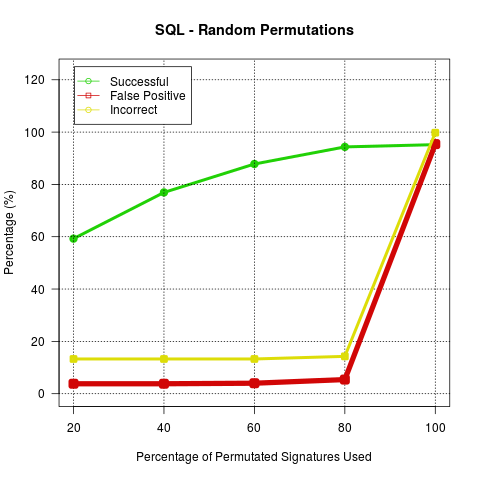
\includegraphics[width=350px]{./assets/results/rand/Results_SQL.png}
	\caption{Permutation of Bitstrings to Detect SQLi}
	\label{fig:resRand}
\end{figure}

\section{Support Vector Machine}

For the testing of the support vector machine it was not nessecary to average together multiple results as there are no random elements in the algorithm and so the same results are produced everytime.  All tests used the same testing data to verify the training process as well as the same training data whenever the required amount of requests did not exceed the amount of used in the genetic algorithms training set.  When doing the genetic algorithm testing it was possible to measure changes by adjusting the algorithm's parameters but in the case of the SVM this is not the case and so instead the training data will be manipulated to observe the changes in performance.

\begin{table}
	\begin{tabular}{|p{2.0in}|p{1.125in}|p{1.125in}|p{1.125in}|}
	\hline
	\textbf{Test} & \textbf{\# of requests of intended detection type} & \textbf{\# of requests of incorrect detection type} & \textbf{\# of requests of non-attacks} \\ 
	\hhline{|=|=|=|=|}
	\textbf{GA Compairson (30\%/30\%/30\%/10\%)} & \textbf{$x$} & \textbf{$2x$} & \textbf{$y$} \\
	\hline
	\textbf{Increasing Non-Threats} & 300 & 600 & \textbf{$x$} \\
	\hline
	\textbf{Increasing Incorrect-Threats} & 300 & \textbf{$2x$} & 350 \\
	\hline
	\end{tabular}
	\caption{Parameters used in each Support Vector Machine Test}
	\label{tab:svmTestParameters}
\end{table}

\newpage
\subsection{Comparison with Genetic Algorithm} \label{sec:resComparison}

The first results are obtained by using the same proportions of attack types used in the genetic algorithm training set of 30\% for each attack type and 10\% remaining is non-threats. The purpose of this test is to create as fair a comparison as possible with the genetic algorithm (Figure \ref{fig:resComparison}).  The output classifier for the best performing instance of each kernel is also included (Figure \ref{fig:resClassifiers}).

\begin{figure}[hb]
	\centering
	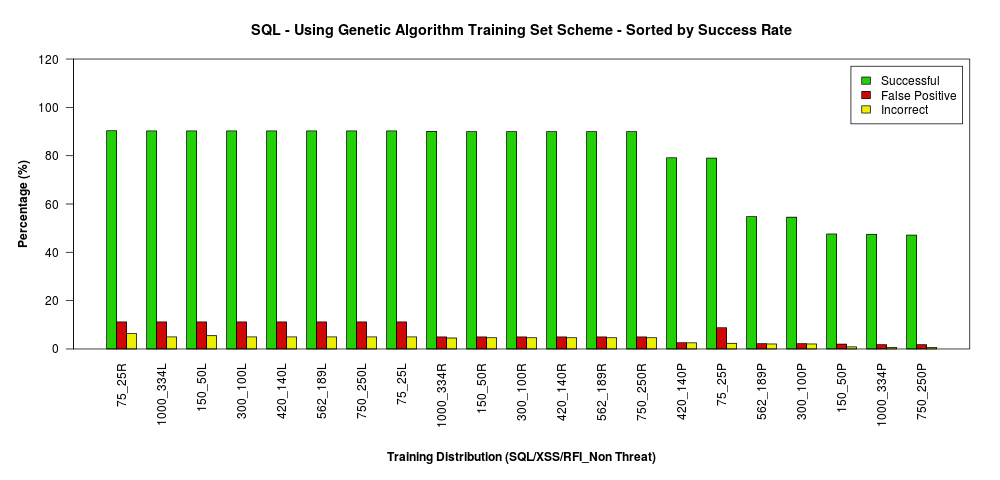
\includegraphics[width=450px]{./assets/results/svm/comparison/Results_SQL.png}
	\caption{Genetic algorithm and SVM comparison for SQLi}
	\label{fig:resComparison}
\end{figure}

\begin{figure}[hb]
	\centering
	\subfloat{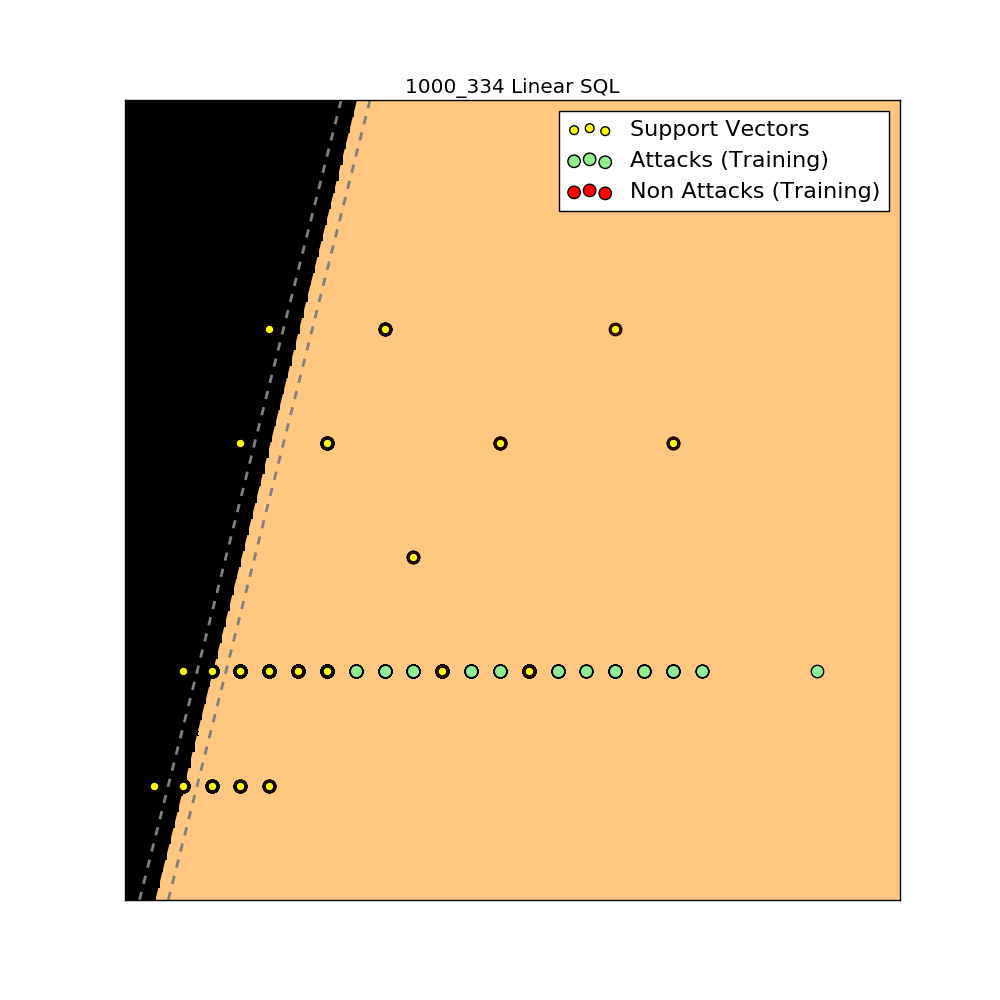
\includegraphics[width=150px]{./assets/results/svm/comparison/linear.png}}
	\subfloat{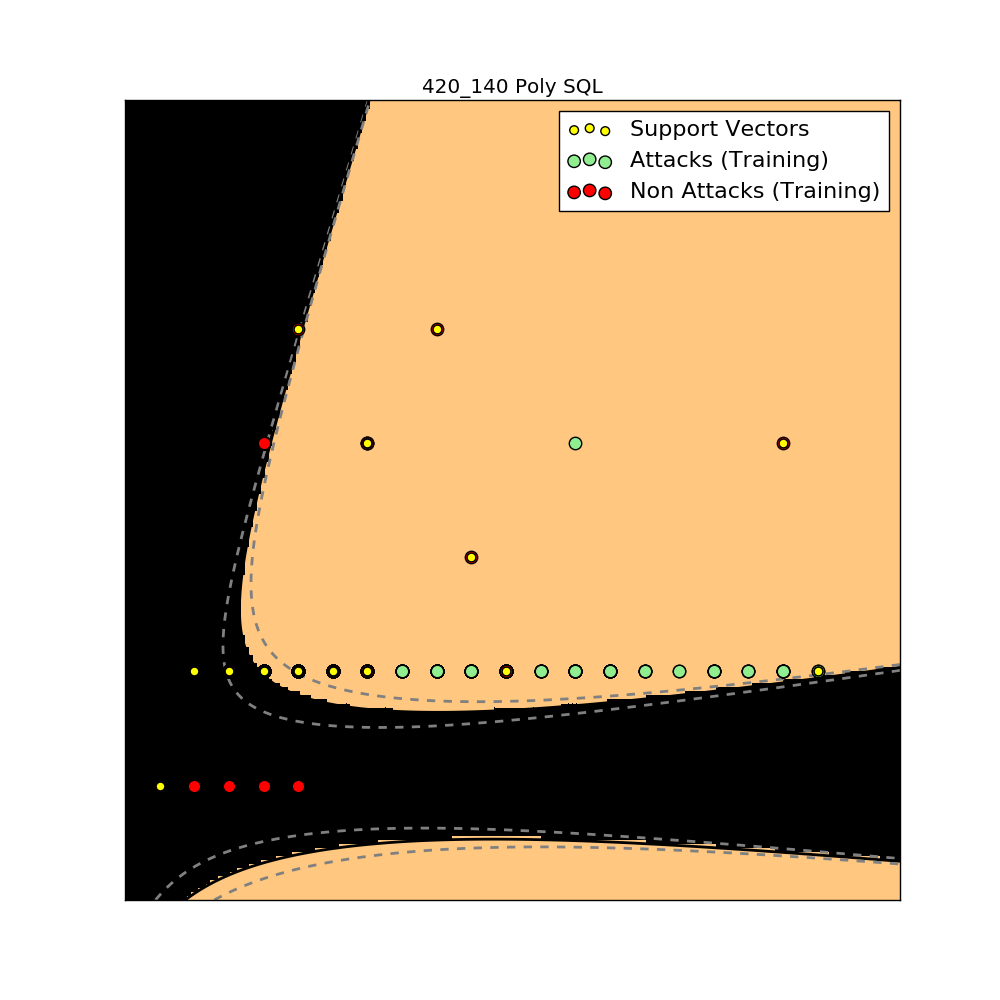
\includegraphics[width=150px]{./assets/results/svm/comparison/poly.png}}
	\subfloat{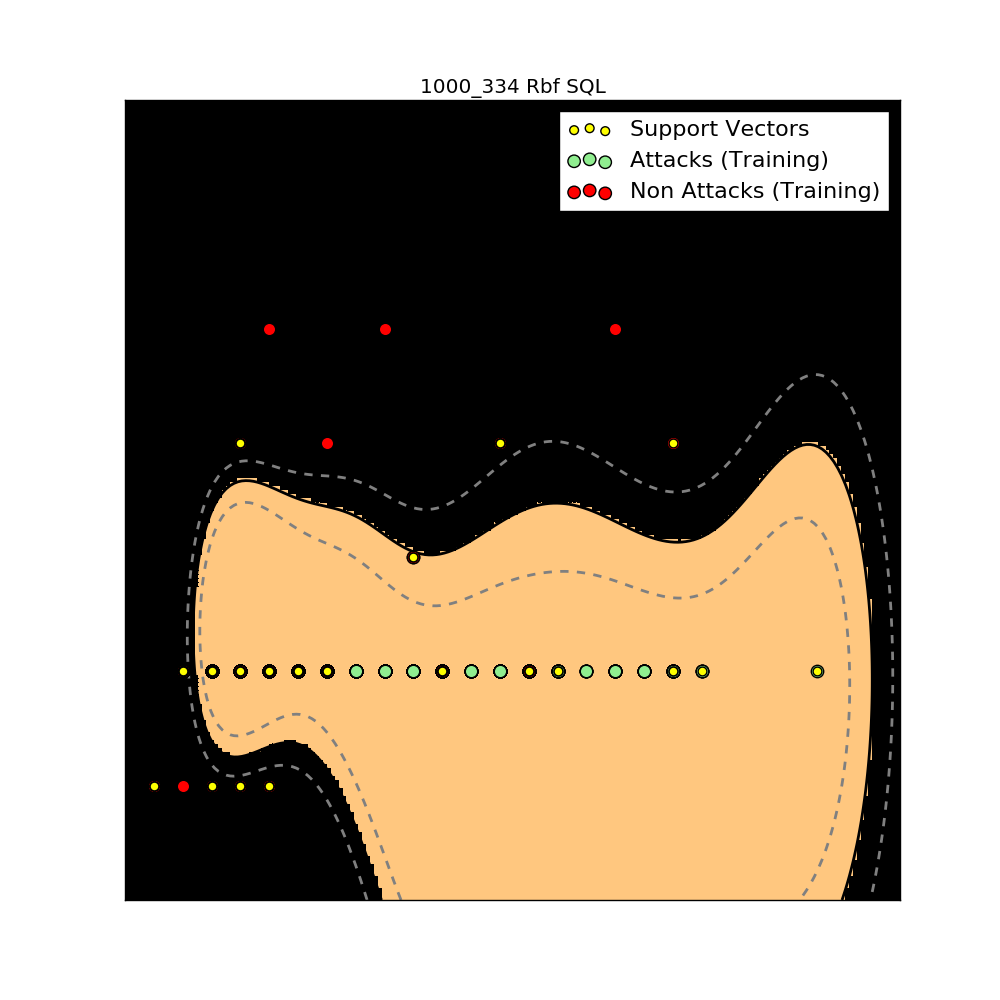
\includegraphics[width=150px]{./assets/results/svm/comparison/rbf.png}}
	\caption{Classifier Output, Linear: 1000\_334, Poly: 420\_140, RBF: 1000\_334}
	\label{fig:resClassifiers}
\end{figure}

\newpage
\subsection{Increasing Non-Threats} \label{sec:resNonThreat}

Increasing the amount of non-threats in the training data should create a classifier that is more resilient to detecting false positives, the more training data the less likely false positives should occur (Figure \ref{fig:resFalse}).

\begin{figure}[hb]
	\centering
	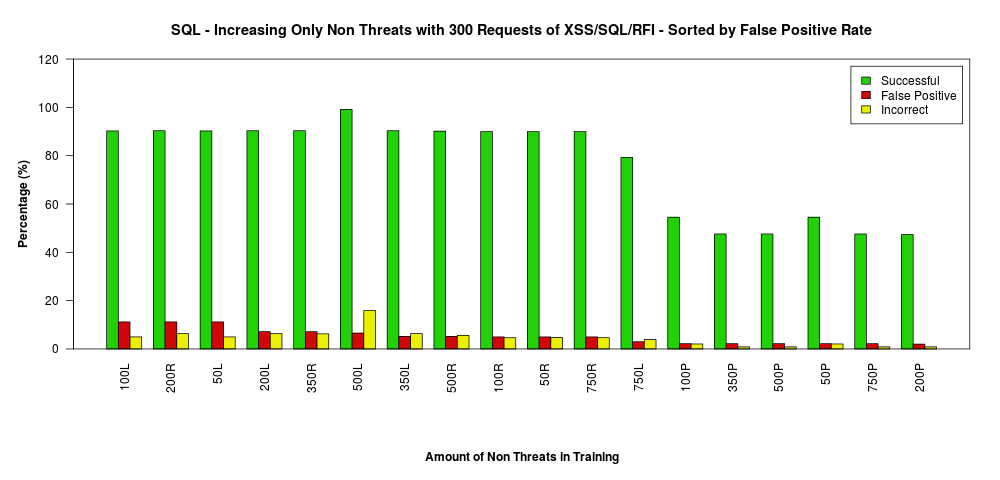
\includegraphics[width=450px]{./assets/results/svm/nonthreat/Results_SQL.png}
	\caption{Effects of increasing non-threat training data in SVM for SQLi detection}
	\label{fig:resFalse}
\end{figure}

\newpage
\subsection{Increasing Incorrect-Threats} \label{sec:resIncorrect}

Similar to the last test, the more threats in the training data that are not the one we are looking for, hopefully the less likely it is for the classifier to incorrectly identify an attack (Figure \ref{fig:resIncorrect}).

\begin{figure}[hb]
	\centering
	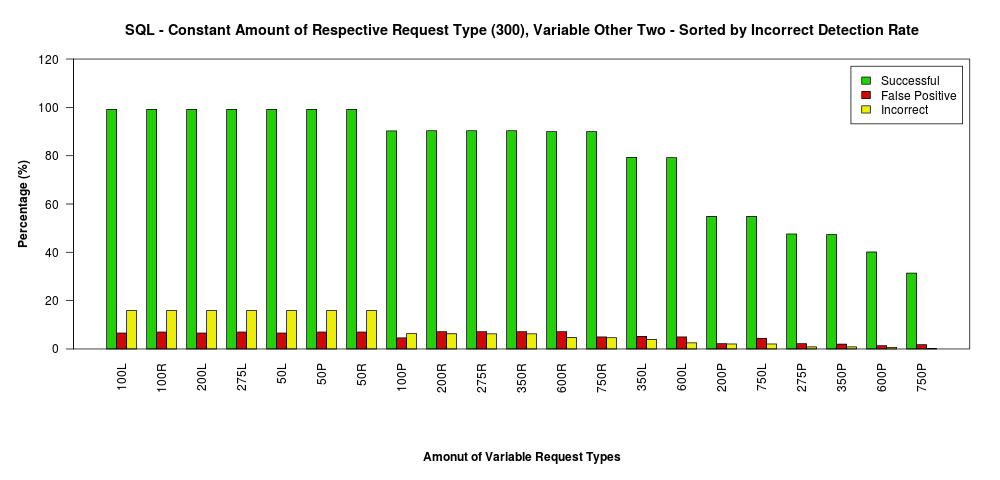
\includegraphics[width=450px]{./assets/results/svm/incorrect/Results_SQL.png}
	\caption{Effects of increasing incorrect attack training data in SVM for SQLi detection}
	\label{fig:resIncorrect}
\end{figure}


